\documentclass[times, utf8, diplomski]{fer}
\usepackage{booktabs}
\usepackage{pdfpages}
\usepackage{catchfile}
\usepackage{xparse}
\usepackage{listings}
\usepackage{nameref}
\usepackage{float}


\renewcommand{\labelitemi}{$\bullet$}

\usepackage{amsthm}
\theoremstyle{definition}
\newtheorem{definition}{Definition}[]

% environment setup
\ExplSyntaxOn
\NewDocumentCommand{\getenv}{om}
 {
  \sys_get_shell:nnN { kpsewhich ~ --var-value ~ #2 } { } \l_tmpa_tl
  \tl_trim_spaces:N \l_tmpa_tl
  \IfNoValueTF { #1 }
   {
    \tl_use:N \l_tmpa_tl
   }
   {
    \tl_set_eq:NN #1 \l_tmpa_tl
   }
 }
\ExplSyntaxOff

\getenv[\resdir]{THESIS_RESDIR}
% done

\newcommand{\pythoncode}[3]{
    \lstinputlisting[xleftmargin=20pt, basicstyle=\small, numbers=left, 
    label=#2, caption=#3, language=Python]{#1}
}

\newcommand{\agtcode}[3]{
    \lstinputlisting[xleftmargin=20pt, basicstyle=\small, numbers=left, 
    label=#2, caption=#3, morekeywords={
        if, else, break, for, while, return,
        fn, struct, let, type,
    }]{#1}
}

\newcommand{\textcode}[3]{
    \lstinputlisting[xleftmargin=20pt, basicstyle=\small, numbers=left, 
    label=#2, caption=#3,
    ]{#1}
}

\begin{document}
\thesisnumber{2568}

\title{Design of a strongly-typed programming language}

\author{Petar Mihalj}

\maketitle

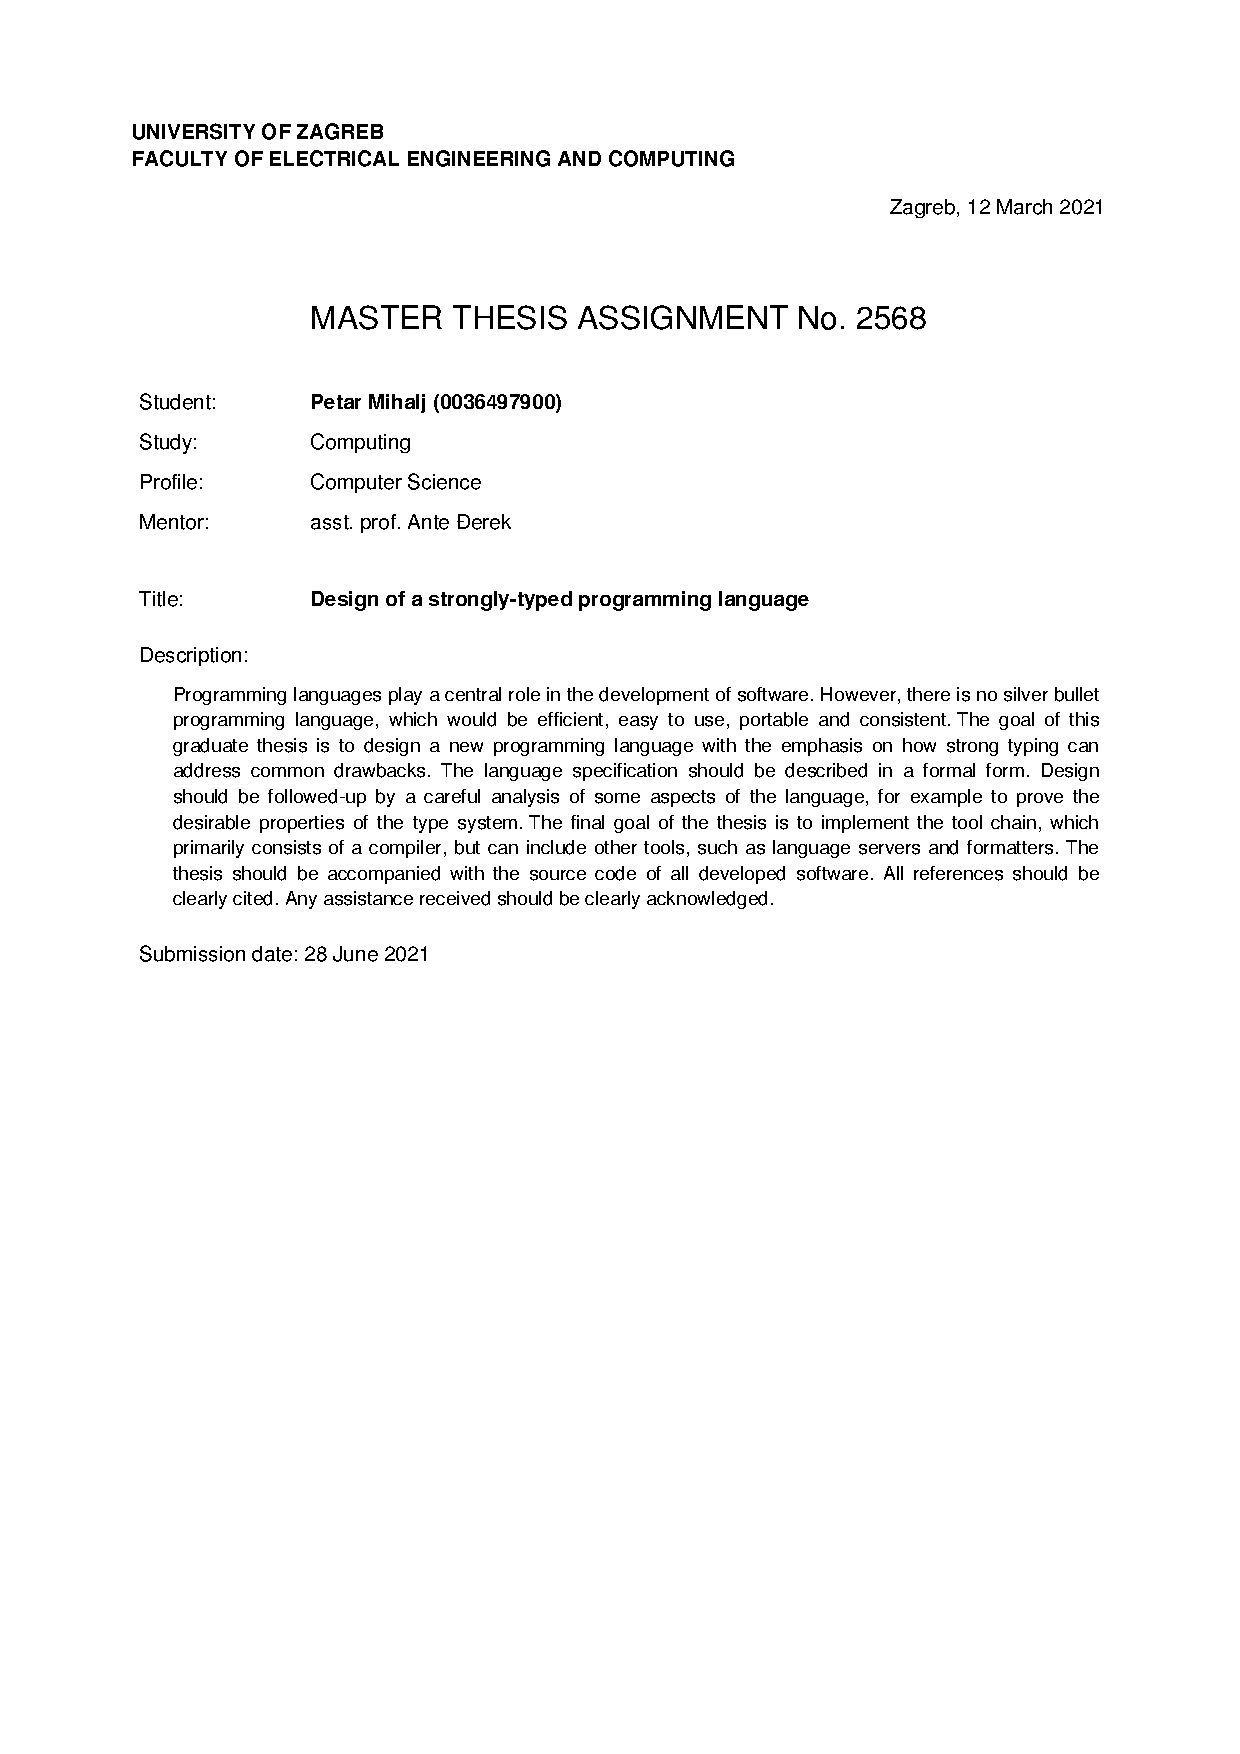
\includepdf[pages={1,2}]{\resdir/task.pdf}

\zahvala{I thank everybody...}

\tableofcontents

\chapter{Introduction}

The programming language developed as a part of this thesis is called AGT.
The name AGT stands for an unfortunate fact that the names of all precious stones
are taken by other programming languages, hence "All Gems are Taken".

\textbf{The AGT programming language} is a statically and 
strongly typed language, with a highly expressive type system.
The type system is used for three main purposes:

\begin{enumerate}
    \item types determine the memory footprint of values 
    \item types allow for polymorphic behaviour of operators and functions on all 
        \textit{concrete types} (built-in or struct types)
    \item type system lets the programmer perform compile-time computation
\end{enumerate}

The language also allows for implementation of object lifetime constructs, 
such as those seen in languages as C++ or Rust; object creation, copying and destruction.

\textbf{The reference AGT compiler (AGTC)} produces executable binaries only.
This is in sharp contrast to some other languages, which can produce object files, 
to later be linked into executables for a particular runtime, 
or used to augument the runtime environment itself (kernel modules, for example). 
This decision was made primarely because the goal of the thesis was to study the language 
from the application programmer's perspective. 
This goal implies that AGT is running on a rich runtime environement, 
where heap memory management and standard I/O are available.
Future updates to AGT specification are meant to allow AGT to be compiled
into linkable files compatible with various platform specific ABIs.

The compiler frontend is implemented using Python3 programming language,
while the backend uses LLVM compiler infrastructure \citep{c_llvm_lattner}.
Allowing for some simplification, AGT is first compiled into LLVM intermediate representation (LLVM-IR),
and than is turned into executable by a chain of tools for compiling LLVM-IR and 
linking the resulting object files into executables.

\section{Example program}

Let us first check out an example AGT program in listing \ref{intro.agt}:

\agtcode{\resdir/programs/intro.agt}{intro.agt}{Example AGT program}

Every AGT program has to have a function definition named main, 
which returns a 32-bit-wide integer,
and has no parameters.
Some functions, like \texttt{outnl}, don't return anything. 
It is important to note that you can't
specify that a function returns \texttt{void} like in C for example.

A \texttt{let <x> = <y>;} construct is an \textit{initialization assignment statement}.
This roughly translates to an allocation of memory on the stack (which can be refered
to as the \textit{location} of <x> from now on), and copying the value of expression <y>
to the location of identifier <x>.

Note that the function call \texttt{in} (line 11) is \textit{parametrized} 
by a \textit{type argument} \texttt{i32}.
Type arguments are used to pass types, but not values. 
They are different than \textit{value arguments}, which carry value too, along with a type.
Note that \textit{passing} of type parameters is purely a compile-time concept;
types can't be refered to during runtime.


The function \texttt{in} is a builtin, and the \texttt{i32} is used to signal the compiler
that we want an instance of this function which returns an \texttt{i32}, 
instead of a \texttt{bool}, for example. 
Of course, user-defined functions can also have \textit{type parameters}, along with \textit{value parameters};
we will get to these later.

Notice that we used the \texttt{cast<i32>} builtin function to convert \texttt{b} to \texttt{i32}
before passing it to function \texttt{mul}. If we didn't do that, the compiler would signal that it can't
compute the expression \texttt{a*b}, since multiplication is predefined only for integer types of same size.
Apart from the \texttt{i8} and \texttt{i32} we used in this example, \texttt{i16} and \texttt{i64} are also
available.

Also, line 6 is terminated by a \texttt{-> a}. This is a return type specification;
it states that this function will return whatever is type of \textt{a}. 

You might have noticed a certain feature while inspecting the code; 
namely the abscence of explicitly stated types in the signature of function definition \texttt{mul}.
While some \textit{dynamically typed} languages (ex. Python) allow for object of any type to be passsed
to the function, AGT behaves quite differently. 

Every time AGTC (AGT compiler) encounters a function call,
it tries to infer a \textit{function type}. Function type is inferred from function definitions. 
Consequently, you can think of the definitions in source code more as \textit{templates} for synthesis
of actual code, than representation of code. 
These definitions lack types, and can't be considered in isolation.
In this example, the call of function \texttt{mul} causes the compiler to try to infer a function type.

Parameters of this \texttt{mul} function definition (\textt{a, b}) can be fit with objects of
any type; it is after this fitting that the compiler will determine that passed types can or can't
be used (due to their incompatibility with a function definition body, for example).

It is important to emphasize that one function definition can be a source of many function types.
The \texttt{outnl} (output with newline) function is a prime example of this behaviour.
It is called three times, with argument of types \texttt{i32}, \texttt{i8} and \texttt{i32}.
Thus, the compiler has to infer two function types, 
one which can be fed with an \texttt{i8}, and one with \texttt{i32}.
The success of this inference corresponds with compilers ability to infer functionality of 
body of the given function definition.

In this case, inference of function definition body will be possible if both function calls on lines
2 and 3 can be inferred. Since \texttt{out} function is a built-in for both \textt{i32} and \textt{i8},
line 2 won't be problematic for inference. Line 3 will be inferred correctly if AGTC suceeds to resolve
function \texttt{out} which takes in an argument of type \texttt{char}. Since this is also a built-in,
inference of function types for both version of \texttt{mul} suceeds.

The property of AGT \textbf{function calls} which can make them refer to different function types, 
when called with different sets of arguments, is called \textit{polymorphism}.
Some sources label polymorphic the very \textbf{function definitions} which, when called upon, 
can result in such behaviour.
We will use these conventions interchangably, since the definition itself is non-rigorous.

Function definition of \texttt{outnl} introduces a special type of polymorphism, 
\textit{parametric polymorphism}. This polymorphic behaviour is said to be present if the
function definition can be a source for potentially unlimited number of types, 
as long as those types are compatible with function definition body.

Python programming language exibits a superficially similar behaviour, but it's
function body compatibility checks occur at runtime. 
The programming style which utilizes this language capability is often called "Duck Typing" 
\citep{c_py_duck_typing}.


\section{Paper organization}

This master thesis will gradually introduce the reader to AGT. 

Chapter 1 has already introduced the reader to basic syntax and semantics,
using a simple example and emphasizing the surface-level properties of type system and inference. 

After the surface-level exploration of the language, chapter 2 will provide an in-depth description of AGT.
This chapter will have many references to the AGTC reference implementation, 
rather than to a separate formal specification. Since AGT is still not a finalized product,
formal specification does not exist, and it's functionality is determined by a reference compiler.
We will mostly focus on the type system, since it is unorthodox and is the main contribution of the author.
Author will justify the decisions which had been made on all levels of AGT design process.

Chapter 3 will supplement the reader with plenty of examples of AGT code. These will
further deepen reader's understanding of AGT. The examples describe impementation
of common programming paradigms, constructs, patterns in AGT, with a detailed explaination
of more esoteric parts of the source code.

In chapter 4 we will address the issues AGT has both on definition and implementation levels,
and discuss the various features that can be improved or added to the language.

Chapter 5 will conclude the thesis and describe future work the author will undertake in order to
improve the language.

%\nameref{chap:main}
\chapter{The AGT Programming Language}\label{chap:main}

AGT compilation process consists of 4 main phases: 

\begin{enumerate}
\item Lexical analysis - tokenization of input source code text
\item Syntactical analysis - rule-based grouping of tokens into an \textit{abstract syntax tree}
\item Semantical analysis - transforming the syntax tree into a \textit{semantical tree}
\item Code generation - inference of the \texttt{main} and code generation
\end{enumerate}

The process is successful if all the steps suceede.

In this chapter we will describe each phase in great detail, contrasting the
newly defined terms against their use in other languages.

\section{Lexical analysis}

The AGT Lexical analysis phase is a standard regular expression parsing process.
Lexical analyzer is fed a stream of characters, which get groupted into tokens,
according to regular expressions and ambiguity resolution rules.

Lexical analyer tool used for the AGTC is PLY - Python Lex-Yacc \citep{c_ply_beazley}.
Python Lex-Yacc is a tool which tries to bring the functionality of well know
lexical and syntactical analyzers Lex and Yacc into Python. The main difference
is that PLY does not \textit{generate} the 
concrete lexer and parser. Instead, PLY user defines the rules fed to PLY by
specifying programming 
constructs like functions that correspond to these rules. PLY then inspects these constructs using 
reflective capabilities of Python, and acts according to these rules
when performing lexical or syntactical analysis.

Let us check out the main lexing module of AGTC, which specifies rules, states and preceedence that
PLY uses to perform lexical analysis for AGT. Some parts of the lexing module
are left out, which is indicated with \texttt{\#...} in source code.

\pythoncode{\resdir/compiler/lexer.py}{}{heyy}

This lexer module has 3 states: \texttt{main} (implicit), \texttt{mlc} (for multiline comments) 
and \texttt{strchar} (for \textit{char arrays} or \textt{char} literals).

Rules for simple operators are given in a string form, 
in a form of \texttt{t\_<TOKEN> = <REGEX>}.

Rules for more tokens which are defined with more complex regular expressions, 
like int literals or identifiers, are defined using functions. 
Those functions can also alter the behaviour of the
lexer when such a token is parsed. For example, whenever an identifier is parsed,
the function \texttt{t\_ID} looks up whether the identifier is in a list of reserved
words, and if it is, changes the token's type. This neat trick greatly simplifies
regular expressions, and is taken from official PLY documentation \citep{c_ply_docs_beazley}.

PLY documentation states that priority is given to regular expressions defined by functions, 
in the order in which they are given.
After function-based rule definitions, 
priority is given to string defined rules (the ones with greater regex length first).

We employ the \textit{state} feature of PLY lexing module, 
which allows us to change the lexer's behaviour
when it encounters, for example, a beginning of a multiline comment. 
In that particular case, lexer goes into \texttt{mlc} state.
When in \texttt{mlc} state, lexer parses and caches every 
symbol until it gets to the end of the comment. 
Both type of comments, \texttt{/*multiline comment*/} and \texttt{//singleline comment} are discarded
after being parsed.

\subsection{Literals}

String and character literals are given in double and single quotes, respectively.
They can include escaped characters:  (\textbackslash 0, \textbackslash n, \textbackslash t, 
\textbackslash ", \textbackslash \textquotesingle). 
Character literal must consist of exactly one character or escaped character.

Integer literals are characterized by both the value and the size of integer containing this value.
Possible integer sizes are 8, 16, 32 and 64.

Example integer literals are:
\begin{itemize}
    \item \texttt{5} (implicitly i32)
    \item \texttt{5i32}
    \item \texttt{516}
    \item \texttt{5i8}
    \item \texttt{5i64}
    \item \texttt{324243} (implicitly i32)
\end{itemize}

Boolean literals are:

\begin{itemize}
    \item \texttt{true}
    \item \texttt{True}
    \item \texttt{false}
    \item \texttt{False}
\end{itemize}

\subsection{Identifiers}

Identifiers consist of a letter or an underscore, followed by any number of letters, underscores or digits.
Reserved words are excluded from identifiers.

Reserved words are:
\begin{itemize}
    \item 'fn', 'struct',
    \item 'let', 'type',
    \item 'if', 'else', 'break', 'for', 'while', 'return',
\end{itemize}


\subsection{Operators}

We will now list the operator families, without discussing their semantics in detail, because

\begin{itemize}
    \item Built-in versions of these operators will be listed in later chapters, and the reader
        can intuitively reason about which ones are available.
    \item User-defined versions of these operators can adhere to a number of different semantics 
        (which is not recommended, but is possible).
    \item Operators can be applied on types during compile time (to produce other types). 
        This discussing is better to be left to later chapters.
\end{itemize}

Apart from the operators themselves, we will list their special names. These names
will be used to translate operator applications to function calls. For example, when 
\texttt{+} is applied to value \texttt{3} and \texttt{5} (\texttt{3+5}), compiler
will insert a call to \texttt{\_\_add\_\_(3,5)} instead. This method derived from operator's special name
is an example of what we call a \textit{dunder} or \textit{magic} method (according to Python folklore).
\textit{Dunder} comes from double-underscore which both preceeds and follows the special name.

\begin{table}[H]
\begin{tabular}{ccc}
\textbf{Arithmetic operators} & \textbf{Comparison operators} & \textbf{Boolean operators} \\
+ (add)                       & == (eq)                       & \& (and)                   \\
- (sub)                       & != (ne)                       & | (or)                     \\
* (mul)                       & \textgreater{}! (gt)          & $\sim$(not)                \\
/ (div)                       & \textless{}! (lt)             &                            \\
\% (mod)                      & \textgreater{}= (ge)          &                            \\
                              & \textless{}= (le)             &                           
\end{tabular}
\end{table}

Note that, even though we call the last group the \textit{boolean} operators,
those operators can be evaluated on operands which are not booleans,
as long as the corresponding dunder functions are defined in the program.

The same goes for arithmetic and comparison operators; a programmer can use
builtins functions for all integer types, but can define additional dunder functions
for \texttt{rectangle} objects, for example.

\subsection{Special operators}

Special operators can't be user-defined, and have a fixed meaning:

\begin{itemize}
    \item \textit{Address of operator} (\textt{@}) can be used on any L-value (explained
        in later chapters), and evaluates to a pointer to that value. For
        example, if \texttt{i} is an \texttt{i8}, then \texttt{@i} is a pointer
    to \texttt{i8}. We can also denote this pointer as \texttt{@i8} - exactly the way it can be used in 
    the context of a type. For example, if you want to check whether a function argument is of \texttt{@i8}
    type (to get polymorphic behaviour), you would start this function with a line:
    \texttt{type \_ = enable\_if<arg == @i8>;}.

    \item Dereference operator (\texttt{!}) can be used on any pointer value, 
        and evaluates to a value which is being pointed to.
        For example, if \texttt{p} is an \texttt{@i8}, then \texttt{p!} is a value of type \texttt{i8}.
    This operator can also be used in the context of a type.
    For example, if you want to check whether a function argument is a pointer (to whatever type), 
    and capture the pointed-to type, you would start this function with a line:
    \texttt{type pointed\_to = enable\_if\_resolve<arg!>;}.
    A new special type expression \texttt{enable\_if\_resolve<...>} exibits similar behaviour as
    \texttt{enable\_if<...>}, in sense that it lets you create polymorphic behaviour. This one will
    succeed if the argument is successfully evaluated (it doesn't have to evaluate to \texttt{i1}).
    If it succeeds, it will also act as if it wasn't there. In this case, 


    \item Index (bracket) operator must be used on a pointer, and be given any integrer type as an argument.
        It will offset the pointer depending on the underlying type. For example, 
        if \texttt{p} is a \texttt{char} pointer, \textt{p[5]} will evaluate to a pointer 
        with a location $lp+5\cdot s$, where $lp$ is \texttt{p}'s value and $s$ is size of char type.
\end{itemize}

Precedence rules of operators will be stated in section 2.2. 
An interested reader will find more details concrening the implementation in
the source code supplied with this paper.


\section{Syntactical analysis}

Syntactical analysis is achieved with a LALR parser implemented in PLY package. 

Tokens resulting from lexical analysis are fed into a stack machine which,
depending on the state of the top of the stack and next token in the list,
either pushes the next token on top of the stack (\textit{shift}) or converts
a number of tokens on the top of the stack to another token (\textit{reduce}).

The grammar rule specifications are given in a different way than the
one standard for PLY. PLY uses functions by default, while AGTC uses
classes which have to adhere to certain structure. These class definitions
are turned into functions (using reflective programming) and finally
dynamically inserted into syntactical parser class definition.
A reader who is interested in details can consult the source code.

The output of a syntactical analysis phase is an abstract syntax tree - a tree structure
which denotes applications of grammar rules to tokens. An example syntax tree, which
results from the statement \texttt{let n = in<i32>();} is given:

\textcode{\resdir/compiler/ast}{}{a}

This tree consists of a single statement. We won't get into details of the semantics here,
since there is a another step which will contextualize the syntax tree and resolve some ambiguities,
which couldn't have been resolved with a LALR parser (which PLY uses).

An example of a rule which is used to generate binary expression nodes is:

\textcode{\resdir/compiler/rule.py}{}{a}

The shift/reduce conflicts of arithmetic expressions are resolved by specifying
a list of operator priorities.

\section{Semantic analysis}

The need for semantical analysis is caused by a fact that AGT's syntax is highly contextual,
that is, expressions that appear in one place can have a radically different meaning
than same expressions which appear in another place.

For example, in the following code snippet, the expression \texttt{a} is used in two distinct contexts.

\textcode{\resdir/compiler/ast}{}{a}

In the ending of the first line, \texttt{a} is a type expression, that is, a compiler is required to produce
a type (which the function returns). In the second line, \texttt{a} is a value expression,
which means compiler is required to produce a value of that expression, rather than a type.
We haven't yet specified what means to produce either a type or a value, but those implementation
details will be dealt with in the next chapter.

What is important for the understanding of AGT is that 

\textcode{\resdir/compiler/diff.py}{}{a}





\section{Type inference}

Type inference is the most complex phase of AGT compilation process.
Before we go heads first into it's description, we will lay down some definitions
and motivate them. Type inference also includes LLVM-IR generation. 

AGT's type inference engine works as a functional programming language,
in a sense that it has to evaluate \textit{type requests}.
This evaluation is \textit{pure}; repeated evaluations always yield the same result.
In a sense, the type engine is a box which provides two evaluation functions.

\section{Concrete type request}

The first function is a \textit{Concrete type request} (CTR). This function maps
a name and a list of concrete types (\textit{type arguments}) into a new concrete type. For example,

\begin{enumerate}
    \item CTR("char", []) -> CharType
    \item CTR("i32", []) -> IntType(32)
    \item CTR("rectangle", [i32]) -> RectangleType(with i32 side lengths)
\end{enumerate}

How does the type engine achieve this mapping? 

One way is to use \texttt{concrete type generators}.
They take CTR arguments and decide whether they can provide a type, for example,
a bool type generator can check whether the name is equal to "bool" and whether 
there are no supplied type arguments; if both conditions are satisfied,
it can provide the concrete type.

The other way is to iterate over user-supplied struct definitions.
For every struct definition whose name matches the supplied name, 
and whose number of type parameters matches the number of supplied type arguments,
the inference is being done. Every sucessful inference is considered in a final decision.

Inference using struct definitions consists of evaluating the body of struct definition,
which might need recursive calls to type engine itself. We ensure that these
recursions are taken care of; for example, recursive structure definitions will fail.

When both of these methods finish, there has to be \textbf{exactly one} candidate type,
otherwise, we have an ambiguity, which is an error.


\section{Function type request}

The second inference function is a \textit{Function type request} (FTR). This function maps
a name and \textbf{two} lists of concrete types (\textit{type arguments} and \textit{value arguments}) 
into a new concrete type. For example,

\begin{enumerate}
    \item FTR("main", [], []) -> FunctionType
    \item FTR("fibonacci",[], [i32]) -> FunctionType
    \item FTR("power", [fast], [i32, i32]) -> FunctionType
    \item FTR("power", [slow], [i32, i32]) -> FunctionType
\end{enumerate}

A FunctionType is a rather complex type; it needs to have all information needed for code synthesis, 
including LLVM code and return type. 

By default, every function call is preceeded by copying of its arguments. However, some built-in functions,
like copy functions of pointers, should not copy their arguments (because of infinite recursive loops).
Only builtin functions can ignore this copying behaviour, and the flag which indicates
whether to do so is also a part of a FunctionType.

Let us take a look at the following code snippet, which demonstrates a sort of polymorphic behaviour.

\textcode{\resdir/compiler/inf1.agt}{}{a}

Suppose the type engine is invoked to fulfill a FTR("power", [slow], [i32, i32]).
Since "power" is not in builtin functions, TE will resort to using function definitions.

When TE starts to infer a type from the definition at line 4, it will immidiatelly encounter a special
construct \texttt{enable\_if<...>} at line 5. This construct is the main driver of polymorphism in AGT.
AGTC will first evaluate it's argument, \texttt{T==slow}, which will resolve to \texttt{i1} (equivalent of
true when used in type context). Enable\_if will, since its argument represents truth, act as if didn't exist;
it will just assign the type to variable on the left side. Since the variable is a \textit{discard token}
(\texttt{\_}), the type won't be assigned, but rather discarded.

The user has achieved polymorphic selection using enable\_if. He signalled the compiler that this
definition of \typett{power} function fits programmers intentions.

On the other hand, consider the definition of \texttt{power} at line 9.
In this line, \texttt{enable\_if} argument will evaluate to \texttt{i0} (false in type context).
This will cause the TE to abandon this function as a potential candidate for type resolution.
Note that this behaviour is not a \critical error (the one which AGTC reports as a mistake),
but rather a mechanism for polymorphic selection.

\section{Lifetime semantics}

Lifetime semantics is a broad term which rougly encompasses the following aspects of objects
in programming languages:

\begin{enumerate}
    \item Objects exist in a specific context, which is dependant on their 
        \subitem lexical environment (the scope)
        \subitem runtime (the function invocation)

        For example, parameters of the function exist and can be referenced throughout the function body,
        but stop existing when that specific invocation of the function terminates. 

    \item The context in which objects exist is called their \textit{lifetime}
    \item Object's lifetime starts with \textit{initialization} (\textit{construction} in some sources).
        \subitem Having precise control over construction can allow programmer
                to restrict usage of the object or set up invariants
    \item Object's lifetime ends with \textit{destruction}.
        Having precise control over destruction allows programmer to
        deconstruct complex inner workings of the object, without relying on programmer to do it manually.
        For example, objects can \textit{release} their resources when they stop existing.
    \item Transferring or duplicating object's contents to other memory location can also be controlled,
        via \texttt{copy operation}. This allows us to, for example, deep copy the memory array, 
        instead of shallow copying the pointer and thus incidentally creating unwanted memory aliases.
\end{enumerate}

Various other semantics can be implemented on top of lifetime model, we will check out an example called
\texttt{Ownership semantics} in the last section. Now we will describe how lifetime semantics fit into
definition of AGT. Before we get into the details though, we have to throughly define types of values.

\begin{definition}[L-value]
A value expression is said to a L-value, 
if the value it evaluates to \textbf{can} be referred to from other context.
\end{definition}

\begin{definition}[R-value]
A value expression is said to a R-value, if it is not L-value, that is
if the value it evaluates to \textbf{can't} be referred to from other context.
\end{definition}

For example, every statement \texttt{let <v> = ...} creates a new memory location,
so the expressions \texttt{<v>} following it and refering to same identifier \texttt{<v>} are lvalues.

On the other hand, function call expressions such as \texttt{gcd(3,2)} are rvalues; their result
(function return value) can't be refered to from any other place, apart from this one.

The distinction between L-values and R-values is crucial when reasoning about copy operations.
Since R-values can't be refered to from any other context, instead of copying their value, 
we can \texttt{memory copy} their value. The crucial distinction is that \texttt{copying}
involves calling the \texttt{copy} function (which might be very expensive, for example for vectors),
and \textit{memory copying} does not copies only the literal memory contents.

\begin{definition}[Initializer]
An initializer is a function whose name is \texttt{__init__}, and which has atleast one value parameter;
a pointer to type being initialized. Other value parameters are objects which are needed for initialization.
\end{definition}

\begin{definition}[Copy function]
An copy function is a function whose name is \texttt{__copy__}, and which has two value parameters;
first being a pointer to memory being copied to, and second one being a pointer to object copied from.
\end{definition}

\begin{definition}[Destructor]
An destructor is a function whose name is \texttt{__dest__}, and which has only one value parameter;
a pointer to object being destroyed.
\end{definition}

Check out the following program and it's output:

\textcode{\resdir/compiler/lifetime_ex.agt}{}{a}
\textcode{\resdir/compiler/lifetime_ex.out}{}{a}

You can clearly see that we have used \texttt{enable\_if} construct in lifetime functions too.
This is crucial to prevent multiple candidates for different concrete types.

These were the basics of lifetime semantics, we will get to more details in examples section.



\chapter{AGT program examples}

This section of the paper will introduce the reader to AGT by presenting, explaining and contemplating
about example programs.

\section{Limited parametric polymorphism}

Parametric polymorphism is a possibility of function to be called with different sets of argument types.

Check out the following example:
\textcode{\resdir/programs/fib_runtime_recursion.agt}{}{a}

Output:
\textcode{\resdir/programs/fib_runtime_recursion.out}{}{a}


\section{Compile time computation}

Check out the following example:
\textcode{\resdir/programs/fib_compile_time.agt}{}{a}

Output:
\textcode{\resdir/programs/fib_compile_time.out}{}{a}


\section{Ownership semantics}

Check out the following example:
\textcode{\resdir/programs/shared_pointer.agt}{}{a}

Output:
\textcode{\resdir/programs/shared_pointer.out}{}{a}

\section{Memory primitives}

Check out the following example:
\textcode{\resdir/programs/memory_object.agt}{}{a}

\section{Memory allocation}

Check out the following example:
\textcode{\resdir/programs/memory_alloc.agt}{}{a}

\section{Object oriented example}

Check out the following example:
\textcode{\resdir/programs/string_mgmt.agt}{}{a}


\chapter{Future improvements}

\section{References}

\section{Syntactic improvements}

\section{Multiple source file support}

\section{Portability}





\chapter{Conclusion}
Zaključak.

\bibliographystyle{dinat}
\bibliography{literatura}

\begin{sazetak}
Sažetak na hrvatskom jeziku.

\kljucnerijeci{Ključne riječi, odvojene zarezima.}
\end{sazetak}

% TODO: Navedite naslov na engleskom jeziku.
\engtitle{Title}
\begin{abstract}
Abstract.

\keywords{Keywords.}
\end{abstract}

\end{document}
